\section{Implementation}

\subsection{Description}

The main objective of this thesis has been to develop a solution that would notify the user about new entries in Data Tracker.

\subsection{Discussion of implementation choice}
There is a number of possible ways to develop such a solution. In this section I will discuss different implementation options, the advantages and disadvantages of each, as well as why I eventually decided to settle on creating an Android application.

\subsubsection{X-Road service}
Andmejälgija specifications requires databases to implement an X-Road interface, as described in \ref{protocol_desc}, so one option would be to create an X-Road service that would query Andmejälgija data over X-Road. The main advantage of this approach would be the freedom on how to notify the users of changes to the access logs. The service could support various channels of communication, including instant messenger bots, e-mail and others. The list of requirements in order to operate such a service is daunting, however. 

\begin{itemize}
    \item {In order to join X-Road, legal entity is needed}
    \item {Permission has to be requested from every X-Road service you want to query data from}
    \item {As part of X-Road network, you need to operate a Security Server. It can be self-hosted anywhere for testing, but for production you need to have a Hardware Security Module (HSM), in order to be compliant with eIDAS requirements. HSM costs typically around 10000€. Renting a production ready Security server from Telia costs 210€ per month \footnote{\url{https://www.telia.ee/ari/it-teenused/serverid-ja-pilv/x-tee-turvaserver/}}}
\end{itemize}

Satisfying this criteria is difficult and expensive. Additionally, even if I succeeded, people would have to consent and entrust me with their data in order to be able to use the solution.

\subsubsection{Standalone approach}
This approach uses Eesti.ee session for accessing Andmejälgija data. Once the user is logged in on eesti.ee state portal, certain internal API endpoints become available. Namely GET https://www.eesti.ee/andmejalgija/api/v1/usages endpoint can be used to query Andmejälgija data. The endpoint requires a parameter dataSystemCodes with which specific databases can be specified. For example GET request /usages?dataSystemCodes=digiregistratuur\&dataSystemCodes=rahvastikuregister would request access logs from Digiregistratuur and Rahvastikuregister.

The main advantage of this approach is the abscence of all disadvantages of the X-Road approach: there is no need for any kind of bureaucracy and the solution could be an open-source project, available for anybody to compile and use. There arises a problem, however. What about the notification part? Do I expect users to set everything up on their hardware, including relevant communication channels? That would narrow down the project's user base to technical people knowing how to self-host, and having a server.

That's why I thought that creating a mobile app would be the most optimal approach. The app would keep the eesti.ee session alive and poll the Data Tracker API. This approach would combine the ease of setting up and use with solution remaining standalone, without a central server.

\subsection{Development}

First of all I had to determine how feasible and reliable the standalone approach would be, especially as I was dealing with user-facing service that I would have to effectively reverse-engineer. The main challenge was to keep the session alive for as long as possible,

The eesti.ee session is established using one of strong authentication methods via TARA authentication service. Once the user is authenticated using ID-card, Mobile-ID, Smart-ID, or eID solution of another EU country, a JWT token is issued, valid for 30 minutes. Once the user is authenticated, certain internal API endpoints become available, including those for refreshing JWT token and getting Data Tracker access logs. The JWT refresh endpoint returns Set-Cookie headers that include an updated JWTTOKEN on success, with updated expiration date (30 minutes from the moment of extention).

In order to test whether the session could be kept alive indefinitely I used Tab Reloader extention for Firefox by James Fray \footnote{\url{https://addons.mozilla.org/en-US/firefox/addon/tab-reloader/}}. Using the browser extention I set up browser to auto reload tab with JWT token refresh endpoint. After 8 hours of experiment I deemed it a success.

Next step was the development of Android application. I have chosen to develop it using Kotlin programming language due to it being a new standard for developing Android apps as well as it having more expressive syntax and promising faster development speed.

The app is compatible with all Android versions starting from Android 8.1, meaning that it would work on approximately 96.4\% of Android devices according to Android Studio API version distribution chart.

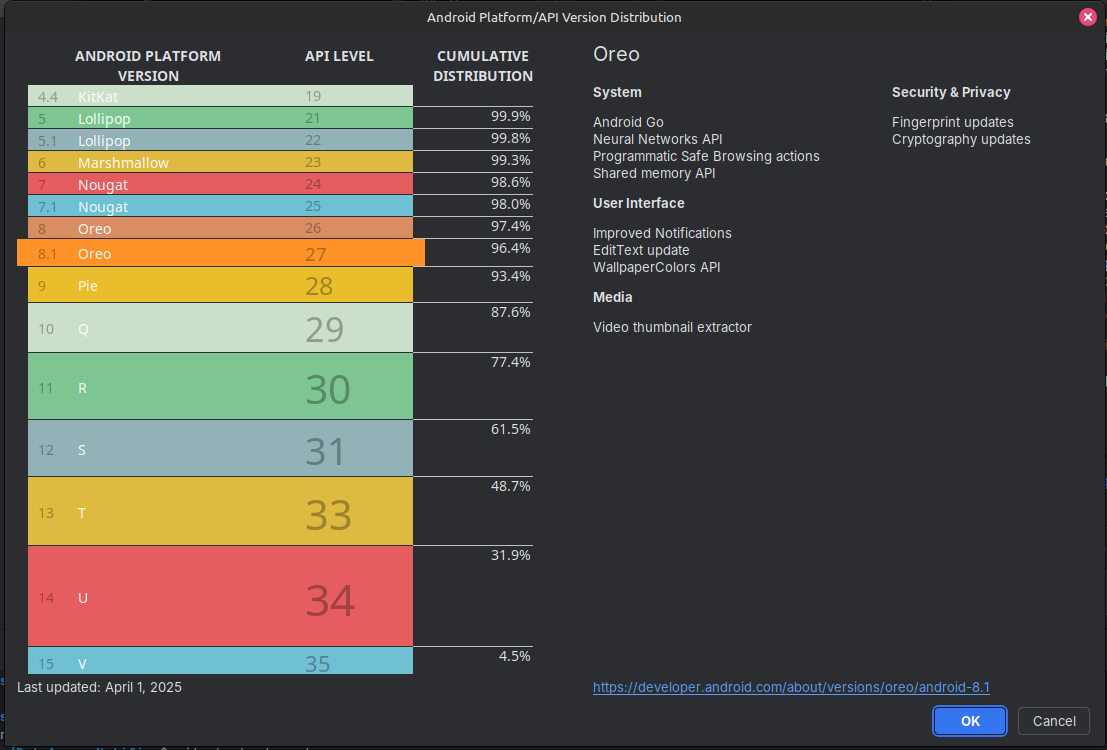
\includegraphics[width=450px]{english/figures/Screenshot from 2025-08-04 19-37-39.png}

The software is open-source, licenced under MIT licence.

At the moment the application support is limited to Android 8.1 and higher. While support for IOS and other platforms is not planned due to limited development time and resources, the author would like to encourage anybody who would deem this solution useful to port it to platforms other than Android.

\subsubsection{Authentication}
In order to get access to eesti.ee internal APIs, the used needs to be authenticated via TARA. An initial plan has been to reverse engineer the authentication flow and authenticate the user by sending raw http requests and sending back responses. This approach, however would be fragile and require substantial engineering effort to develop and maintain.

Instead, I decided to use Android WebView for authentication as a more reliable and convenient approach for both the user and the developer. By leveraging WebView, the app can present the official TARA login page directly to the user, allowing them to authenticate using their preferred method (ID-card, Mobile-ID, Smart-ID, or eID of another EU country). This approach significantly reduces the risk of breaking changes due to updates on the eesti.ee or TARA platforms. Once the user is authenticated, the app can access the necessary session cookies and JWT token to interact with the internal APIs.

\subsubsection{Interacting with eesti.ee internal APIs}
For interacting with eesti.ee internal API I used OkHttp library by Square, Inc. \footnote{\url{https://square.github.io/okhttp/}}. I have used the following API endpoints:

\begin{itemize}
    \item \textbf{GET} \texttt{https://www.eesti.ee/timur/jwt/extend-jwt-session}
    
    An endpoint for extending JWT session.
    
    \item \textbf{GET} \texttt{https://www.eesti.ee/andmejalgija/api/v1/usages}
    
    An endpoint for querying Data Tracker access logs.
    
    Query parameters:
    \begin{itemize}
        \item \texttt{dataSystemCodes}: The name of the information system the access logs are queried from.
    \end{itemize}
    
    \samepage
    Response body format (JSON):
    \begin{small}
    \begin{verbatim}
{
  "findUsageResponses": [
    {
      "logTime": "2025-08-03T22:40:47",
      "receiver": "Tervise ja Heaolu Infosüsteemide Keskus",
      "infoSystemCode": "rahvastikuregister",
      "action": "ISIKU NIME VÄLJASTAMINE ISIKUKOODI PÕHJAL"
    },
    ...
  ]
}
    \end{verbatim}
    \end{small}
    
    Response fields:
    \begin{itemize}
        \item \texttt{logTime}: Timestamp of the data access event in ISO 8601 format
        \item \texttt{receiver}: Registry code of the entity that accessed the data
        \item \texttt{infoSystemCode}: Code identifying the information system
        \item \texttt{action}: Description of the action performed (in Estonian)
    \end{itemize}
\end{itemize}

Both endpoints require a valid JWT token in order to succeed. WebView's CookieManager serves as a single source of truth in this application, where all cookies are loaded from for making requests and written to on responses.

\subsubsection{Keeping the session alive}
The API requests are authenticated using JWT token cookie, the lifetime of which is 30 minutes. This means that the app has to either run a continuous foreground service or be waken up every once in a while in order to request an updated JWT token and send requests to Data Tracker.

On Android there are several ways to accomplish this, although it's worth mentioning that Android is very restrictive regarding background tasks and battery usage. I have tried several approaches and will describe my experience with them in the context of developing this app.

\paragraph{WorkManager}
According to Android documentation WorkManager is the recommended solution for persistent work, Work is persistent when it remains scheduled through app restarts and system reboots. This seemed to describe my use case very well, so that was the first approach that I have tried.

Work is defined in WorkManager using a WorkRequest. There are several WorkRequest types available, including PeriodicWorkRequest and OneTimeWorkRequest.

Using PeriodicWorkRequest, it is possible to schedule periodic tasks. The important limitation here is that it is not possible to schedule a task to execute more frequently than every 15 minutes. While this may sound appropriate for the use case of having to renew the session at least every 30 minutes, in reality things look differently.

During development, I discovered a critical difference between session handling in web browsers versus HTTP client libraries. While the browser-based testing with Tab Reloader successfully maintained the session by refreshing the JWT token every 15 minutes, the same approach using OkHttp in the Android application failed to keep the session alive .

The exact cause of this discrepancy remains unclear. It appears that the eesti.ee session management system expects more frequent interaction or handles cookie management differently when requests originate from HTTP client libraries compared to full web browsers. And indeed, with shorter intervals of 5 minutes the session stays alive. This behavioral difference rendered the PeriodicWorkRequest approach with 15-minute intervals unsuitable for maintaining persistent sessions in the application context.

While OneTimeWorkRequest is meant for one time tasks, it is possible to chain them by having each one-time work create another one-time work at the end of it's lifespan.This approach allows to set custom intervals shorter than 15 minutes, curcumventing the limitation imposed by PeriodicWorkRequest.

While OneTimeWorkRequest may sound like a good solution, WorkManager itself appeared to be rather unreliable for my use case after some testing. The core reason behind limitations to follow is that tasks scheduled by WorkManager are managed by the system and may be deffered if deemed needed by the Android system, for example in the low battery scenario, or even in other scenarios depending on the aggressivenes of the Android variant in regards to the restrictions imposed on the behaviour of the apps.

\paragraph{Foreground Service}
Foreground service is one of the most reliable types of tasks the application can schedule. As opposed to background services, foreground services are considered to be of higher priority to the system and thus are not candidates for being killed when the system is low on memory or the phone is low on battery.

An important limitation has been introduced in the latest Android updates though. More specifically, starting from Android 15, he system places restrictions on how long certain foreground services are allowed to run while your app is in the background. Currently, this restriction only applies to dataSync and mediaProcessing foreground service type foreground services.

The most appropriate foreground service type for my use case is dataSync, meaning that it falls under the 6 hour restriction. While it should be possible to choose an arbitrary foreground service type regardless of the type of an actual task, doing so is not the cleanest approach, especially considering the existance of better alternatives. Furthermore, doing so may also impact the app being accepted into Google Play Store.

\paragraph{AlarmManager + dataSync foreground service}

After evaluating the limitations of WorkManager and the restrictions on foreground services, I ultimately settled on a hybrid approach combining AlarmManager with a dataSync foreground service. AlarmManager is a system service that allows scheduling operations to be executed at specific times, even if the app is not running. By using AlarmManager to trigger the app at regular intervals (e.g., every 5 minutes), I ensure that the session renewal and data polling tasks are reliably executed.

When the alarm fires, the app starts a short-lived dataSync foreground service to perform the necessary network operations: refreshing the JWT token and querying the Data Tracker API. This approach leverages the reliability of foreground services for critical tasks while minimizing battery usage by only running the service when needed. AlarmManager itself is not subject to aggressive background restrictions and can wake the app even in Doze mode, making it suitable for periodic tasks.

This solution proved to be robust and reliable across different Android versions and device manufacturers. Both AlarmManager and foreground services are extremely reliable even on low battery, ensuring that the session remains alive and notifications are delivered promptly to the user.






\subsection{User guide}
\subsection{Software distribution}
\subsection{Known problems}
